\documentclass{beamer} % 使用 beamer 文档类进行幻灯片制作

% 设置主题和颜色等样式 (可选,可以根据喜好选择)
\usetheme{Darmstadt}
\usecolortheme{dolphin}
\usefonttheme{structurebold}

\usepackage{ctex} % 支持中文
\usepackage[utf8]{inputenc} % 设置输入编码为 UTF-8
\usepackage[T1]{fontenc} % 设置字体编码
\usepackage{graphicx} % 插入图片的宏包
\usepackage{grffile} % 支持文件名中的特殊字符,如 _
\usepackage{amsmath} % 数学公式宏包
\usepackage{amsfonts} % 数学字体宏包
\usepackage{amssymb} % 数学符号宏包
\usepackage{hyperref} % 添加超链接

% 设置标题、作者、日期
\title{电力需求数据集探索性数据分析与特征工程} % 报告标题作为幻灯片标题
\author{SakuraPuare} % 作者
\institute{\href{https://github.com/SakuraPuare/ElectricityDemand}{github.com/SakuraPuare/ElectricityDemand}}
\date{\today} % 使用当前日期

\begin{document}

% 标题页
{
\setbeamertemplate{footline}{} % 移除标题页的页脚
\frame{\titlepage}
}

% 目录页
\begin{frame}{目录}
    \begin{columns}[T,onlytextwidth]
        \begin{column}{0.5\textwidth}
            \tableofcontents[sections={1-4}]
        \end{column}
        \begin{column}{0.5\textwidth}
            \tableofcontents[sections={5-10}]
        \end{column}
    \end{columns}
\end{frame}

% ============== 章节内容 ==============

% 引言
\section{引言}
\begin{frame}{引言}
    \frametitle{背景与目标}
    \begin{itemize}
        \item 电力需求预测的重要性
        \item 本报告目标:
        \begin{itemize}
            \item 数据集理解与探索性分析 (EDA)
            \item 数据质量评估
            \item 特征工程构建预测特征集
        \end{itemize}
    \end{itemize}
    % 更多引言内容...
\end{frame}

% 数据集概览
\section{数据集概览}
\begin{frame}{数据集概览}
    \frametitle{数据集结构}
    数据集包含三个主要部分:
    \begin{itemize}
        \item \textbf{电力需求数据 (Demand Data)}: unique\_id, timestamp, y (kWh)
        \item \textbf{元数据 (Metadata)}: unique\_id, location\_id, building\_class, freq, etc.
        \item \textbf{天气数据 (Weather Data)}: location\_id, timestamp, temperature\_2m, humidity, etc.
    \end{itemize}
    % 更多概览信息...
\end{frame}

% 数据量与数据质量分析
\section{数据概览与质量} % 合并并简化标题

% 合并数据量、缺失值、重复值、时间范围到同一页
\begin{frame}{数据概览与质量摘要}
    \frametitle{核心信息速览}
    \textbf{1. 数据量:}
    \begin{itemize}
        \item Demand: ~2.38 亿条
        \item Metadata: 7572 条
        \item Weather: ~60.5 万条
    \end{itemize}

    \textbf{2. 缺失值:}
    \begin{itemize}
        \item Demand: y (~1.3\%) 缺失
        \item Metadata: 位置信息 (~3.1\%) 缺失
        \item Weather: 无缺失
    \end{itemize}

    \textbf{3. 重复值:}
    \begin{itemize}
        \item Demand/Metadata: 无重复
        \item Weather: 极少量重复 (已处理)
    \end{itemize}

    \textbf{4. 时间范围:}
    \begin{itemize}
        \item Demand: 2011-01-01 \(\sim\) 2017-12-31
        \item Weather: 2011-01-01 \(\sim\) 2019-01-01 (覆盖需求数据)
    \end{itemize}
    % 移除了子小节,直接在这一页展示主要质量信息
\end{frame}

% 电力需求分析
\section{电力需求分析}

\subsection{分布特征} % 保留分布特征子节
\begin{frame}{电力需求分布}
    \frametitle{分布形态与异常值}
    \begin{itemize}
        \item \textbf{原始尺度:} 高度右偏 (均值 \(>\)> 中位数),标准差大,存在极端高值。存在少量非正值。
        \item \textbf{log1p 变换:} 改善对称性,更接近正态但仍有峰态。
    \end{itemize}
    \begin{columns}
        \begin{column}{0.48\textwidth}
            \centering
            \begin{figure}
                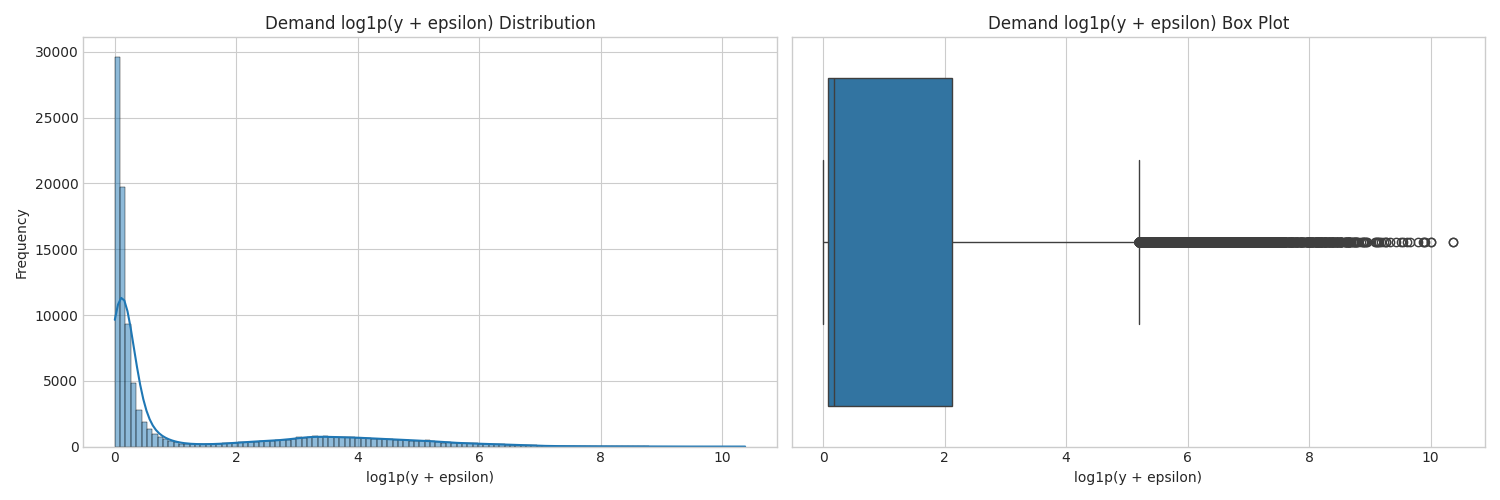
\includegraphics[width=\textwidth]{../plots/demand_y_distribution_log1p_scale.png}
                \caption{log1p 变换分布}
            \end{figure}
        \end{column}
    \end{columns}
\end{frame}

\subsection{时间序列特征} % 保留时间序列特征子节
\begin{frame}{电力需求时间序列示例}
    \frametitle{典型模式与特性}
    \begin{itemize}
        \item 多重周期性 (日内,周内,年度)
        \item 波动性,异常值,趋势性
        \item 不同用户模式多样性 (Residential vs Commercial)
    \end{itemize}
    % 尝试将两个时间序列样本图放在同一页
    \begin{columns}
        \begin{column}{0.48\textwidth}
            \centering
            \begin{figure}
                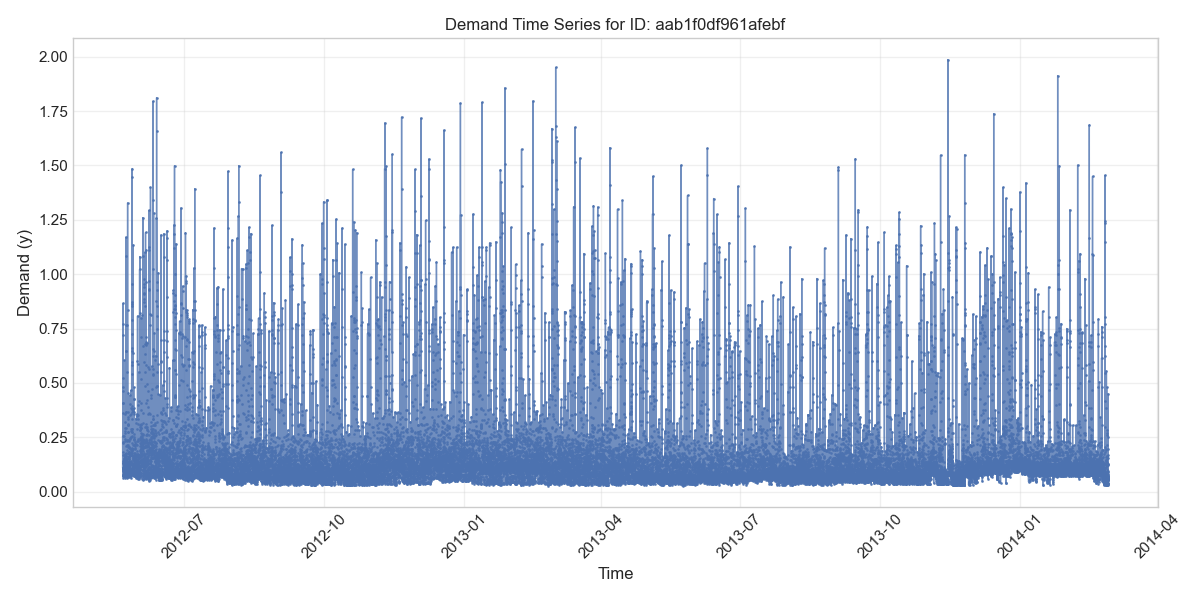
\includegraphics[width=\textwidth]{../plots/timeseries_sample_aab1f0df961afebf.png}
                \caption{样本 1 (日内/周内)}
            \end{figure}
        \end{column}
        \begin{column}{0.48\textwidth}
            \centering
            \begin{figure}
                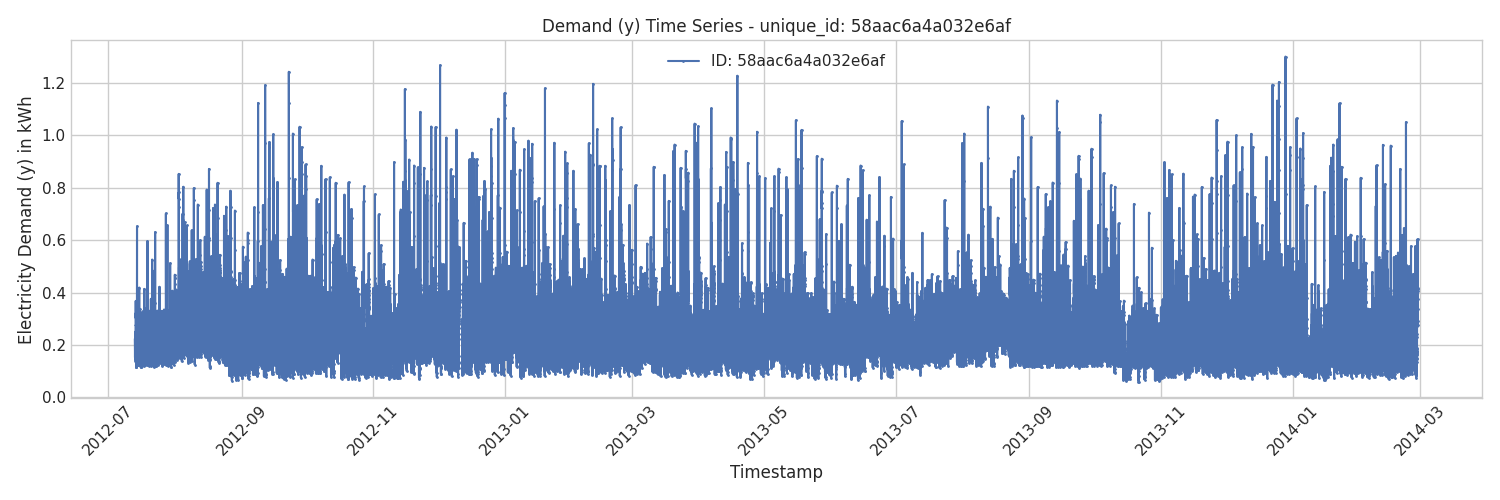
\includegraphics[width=\textwidth]{../plots/timeseries_sample_58aac6a4a032e6af.png}
                \caption{样本 5 (工作日 vs 周末)}
            \end{figure}
        \end{column}
    \end{columns}
\end{frame}

% 元数据分析
\section{元数据分析}
\begin{frame}{元数据分析}
    \frametitle{主要特征分布与地理位置}
    \begin{itemize}
        \item \textbf{分类特征:} Building Class (住宅为主), Location (集中于伦敦), Freq (30T, 1H 为主), Timezone (Europe/London), Dataset Source。
        \item \textbf{数值/地理特征:} 经纬度集中分布,Cluster Size (多数为单个建筑),地理位置有缺失记录。
    \end{itemize}
    % 将两个元数据图放在同一页
    \begin{columns}
        \begin{column}{0.48\textwidth}
            \centering
            \begin{figure}
                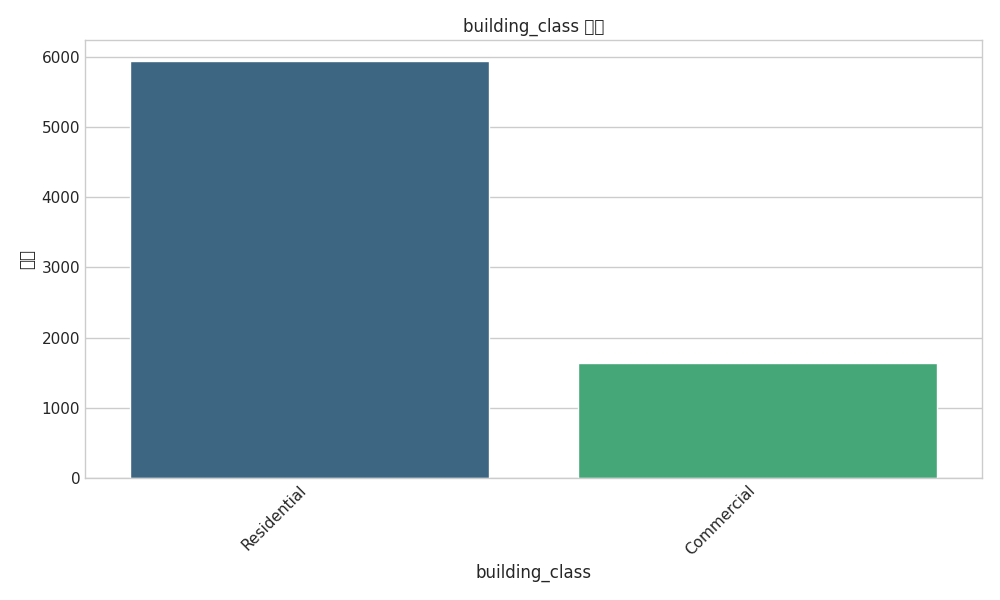
\includegraphics[width=\textwidth]{../plots/metadata_dist_building_class.png}
                \caption{建筑类型分布}
            \end{figure}
        \end{column}
        \begin{column}{0.48\textwidth}
            \centering
            \begin{figure}
                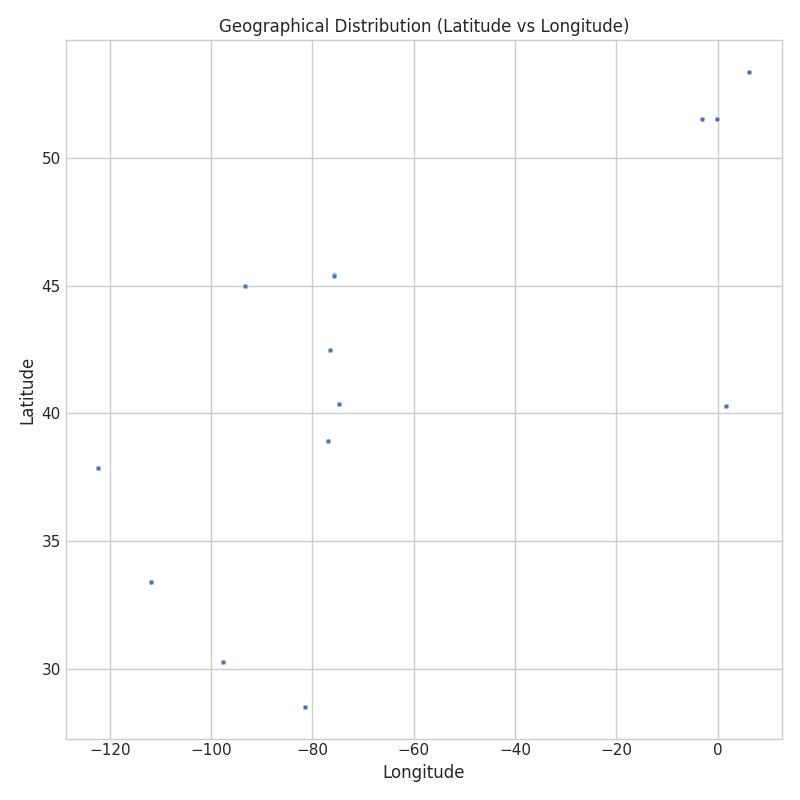
\includegraphics[width=\textwidth]{../plots/metadata_location_scatter.png}
                \caption{监测点地理位置}
            \end{figure}
        \end{column}
    \end{columns}
\end{frame}

% 天气数据分析
\section{天气数据分析}
\begin{frame}{天气数据分析}
    \frametitle{主要天气特征分布}
    \begin{itemize}
        \item \textbf{数值特征:} Temperature (近似正态), Relative Humidity (分布较广), Precipitation (零膨胀), Wind Speed (右偏) 等。
        \item \textbf{其他特征:} Cloud Cover (U 形), Sunshine Duration (两极), Weather Code (常见类型), Is Day (昼夜平衡)。
    \end{itemize}
     % 将两个天气图放在同一页
    \begin{columns}
        \begin{column}{0.48\textwidth}
            \centering
            \begin{figure}
                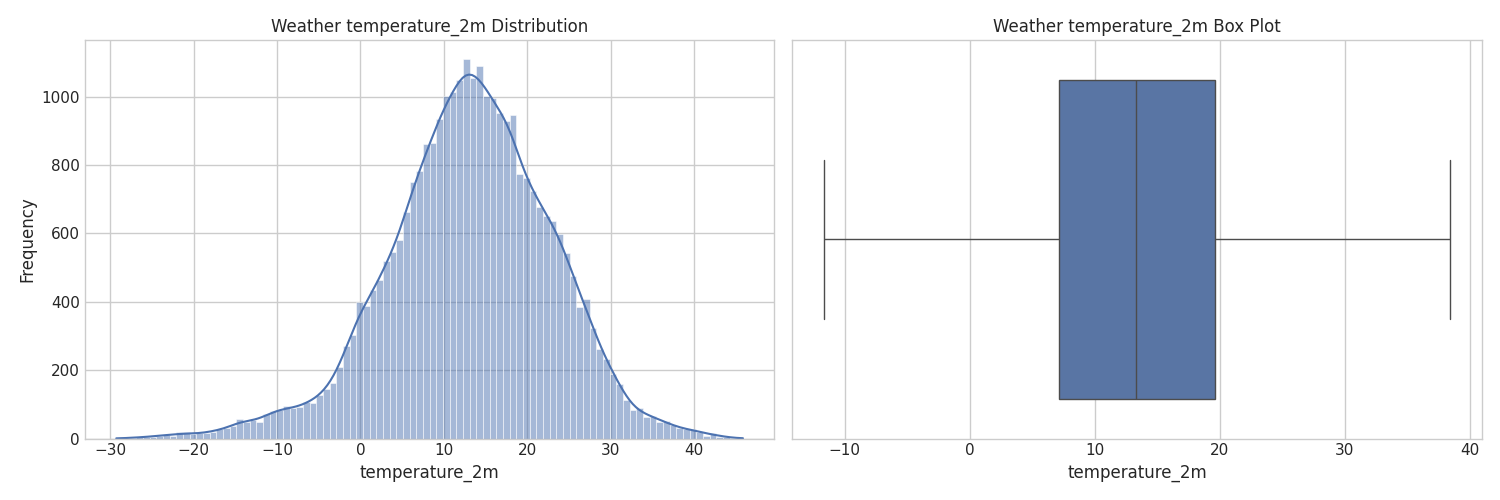
\includegraphics[width=\textwidth]{../plots/weather_distribution_temperature_2m.png}
                \caption{温度分布}
            \end{figure}
        \end{column}
        \begin{column}{0.48\textwidth}
            \centering
                \begin{figure}
                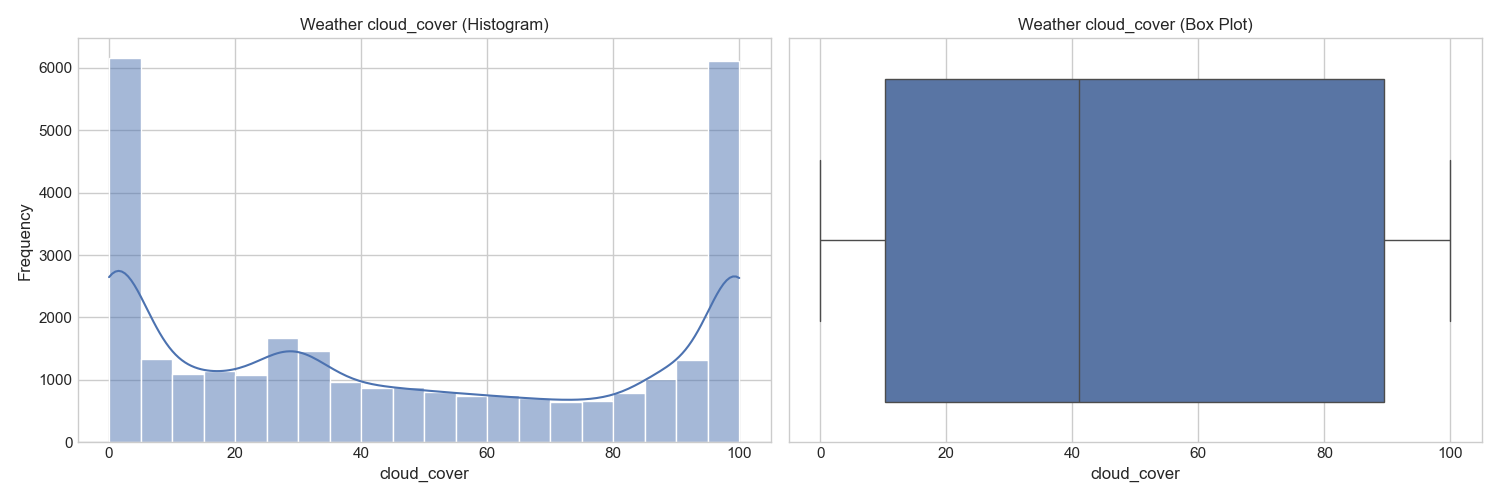
\includegraphics[width=\textwidth]{../plots/weather_distribution_cloud_cover.png}
                \caption{总云量分布}
            \end{figure}
        \end{column}
    \end{columns}
\end{frame}

% 关系分析
\section{关系分析与数据合并} % 合并标题

\subsection{需求与元数据关系} % 保留子节
\begin{frame}{需求与元数据关系}
    \frametitle{建筑类型对需求的影响}
    \begin{itemize}
        \item Commercial (商业) 建筑的电力需求通常显著高于 Residential (住宅)。
        \item 不同 Dataset/Location 的需求分布也存在差异。
    \end{itemize}
    \begin{figure}[H]
        \centering
        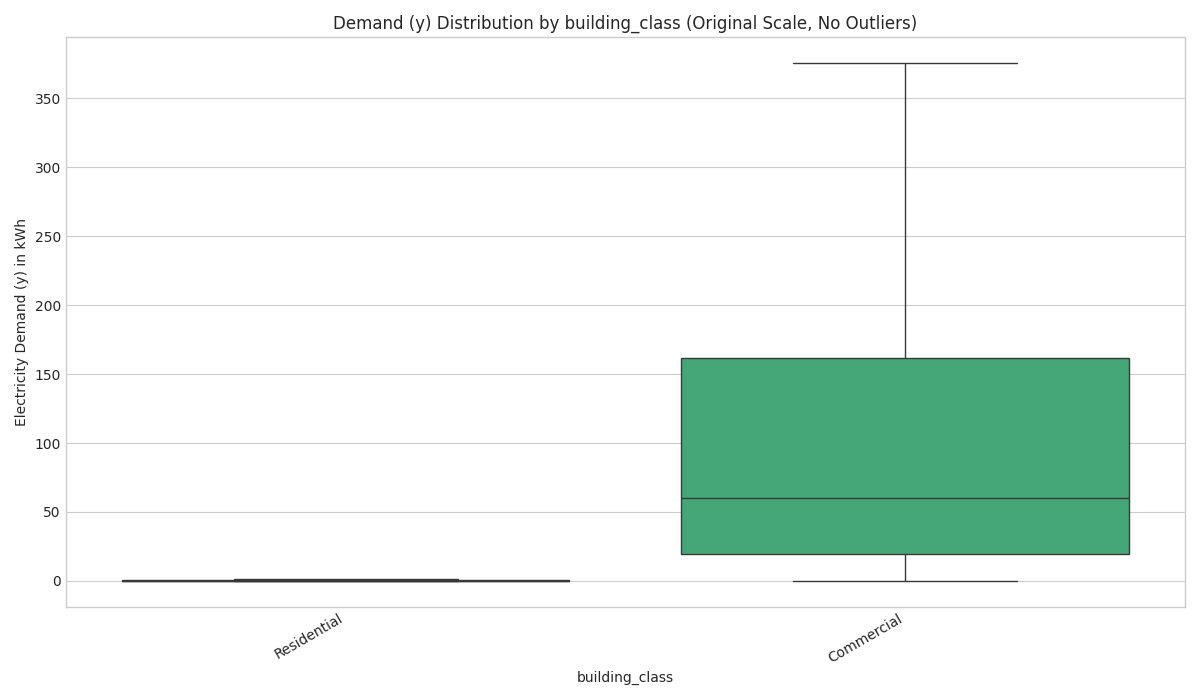
\includegraphics[width=0.6\textwidth]{../plots/demand_vs_building_class_boxplot_orig.png}
        \caption{需求 vs 建筑类型 (原始尺度箱线图)}
    \end{figure}
\end{frame}

\subsection{需求与天气关系及合并} % 合并子节标题
\begin{frame}{需求与天气关系 \& 数据合并}
    \frametitle{相关性与合并流程}
    \textbf{1. 初步相关性:}
    \begin{itemize}
        \item Demand 与 Temperature 弱正相关 (~0.028)
        \item Demand 与 Apparent Temperature 弱正相关 (~0.038)
        \item Demand 与 Relative Humidity 中度负相关 (~-0.202)
    \end{itemize}

    \textbf{2. 数据合并流程:}
    \begin{enumerate}
        \item 加载数据 \& 需求重采样到小时。
        \item 需求 + 元数据 合并 (基于 unique\_id)。
        \item 天气数据去重 \& 时间戳对齐 (到小时)。
        \item 需求/元数据数据 + 天气数据 合并 (左连接 using location\_id, hourly timestamp)。
    \end{enumerate}
\end{frame}

% 数据合并结果和天气相关性矩阵放在下一页
\begin{frame}{数据合并结果与天气相关性}
    \frametitle{合并诊断与天气特征关联}
    \begin{itemize}
        \item \textbf{合并诊断:} 约 1.73\% 记录因 Location ID 缺失/不匹配未能关联天气,其余成功关联。
        \item \textbf{天气特征相关性:} 如下图所示,天气特征内部存在相关性 (例如温度与体感温度高度相关)。
    \end{itemize}
     \begin{figure}[H]
        \centering
        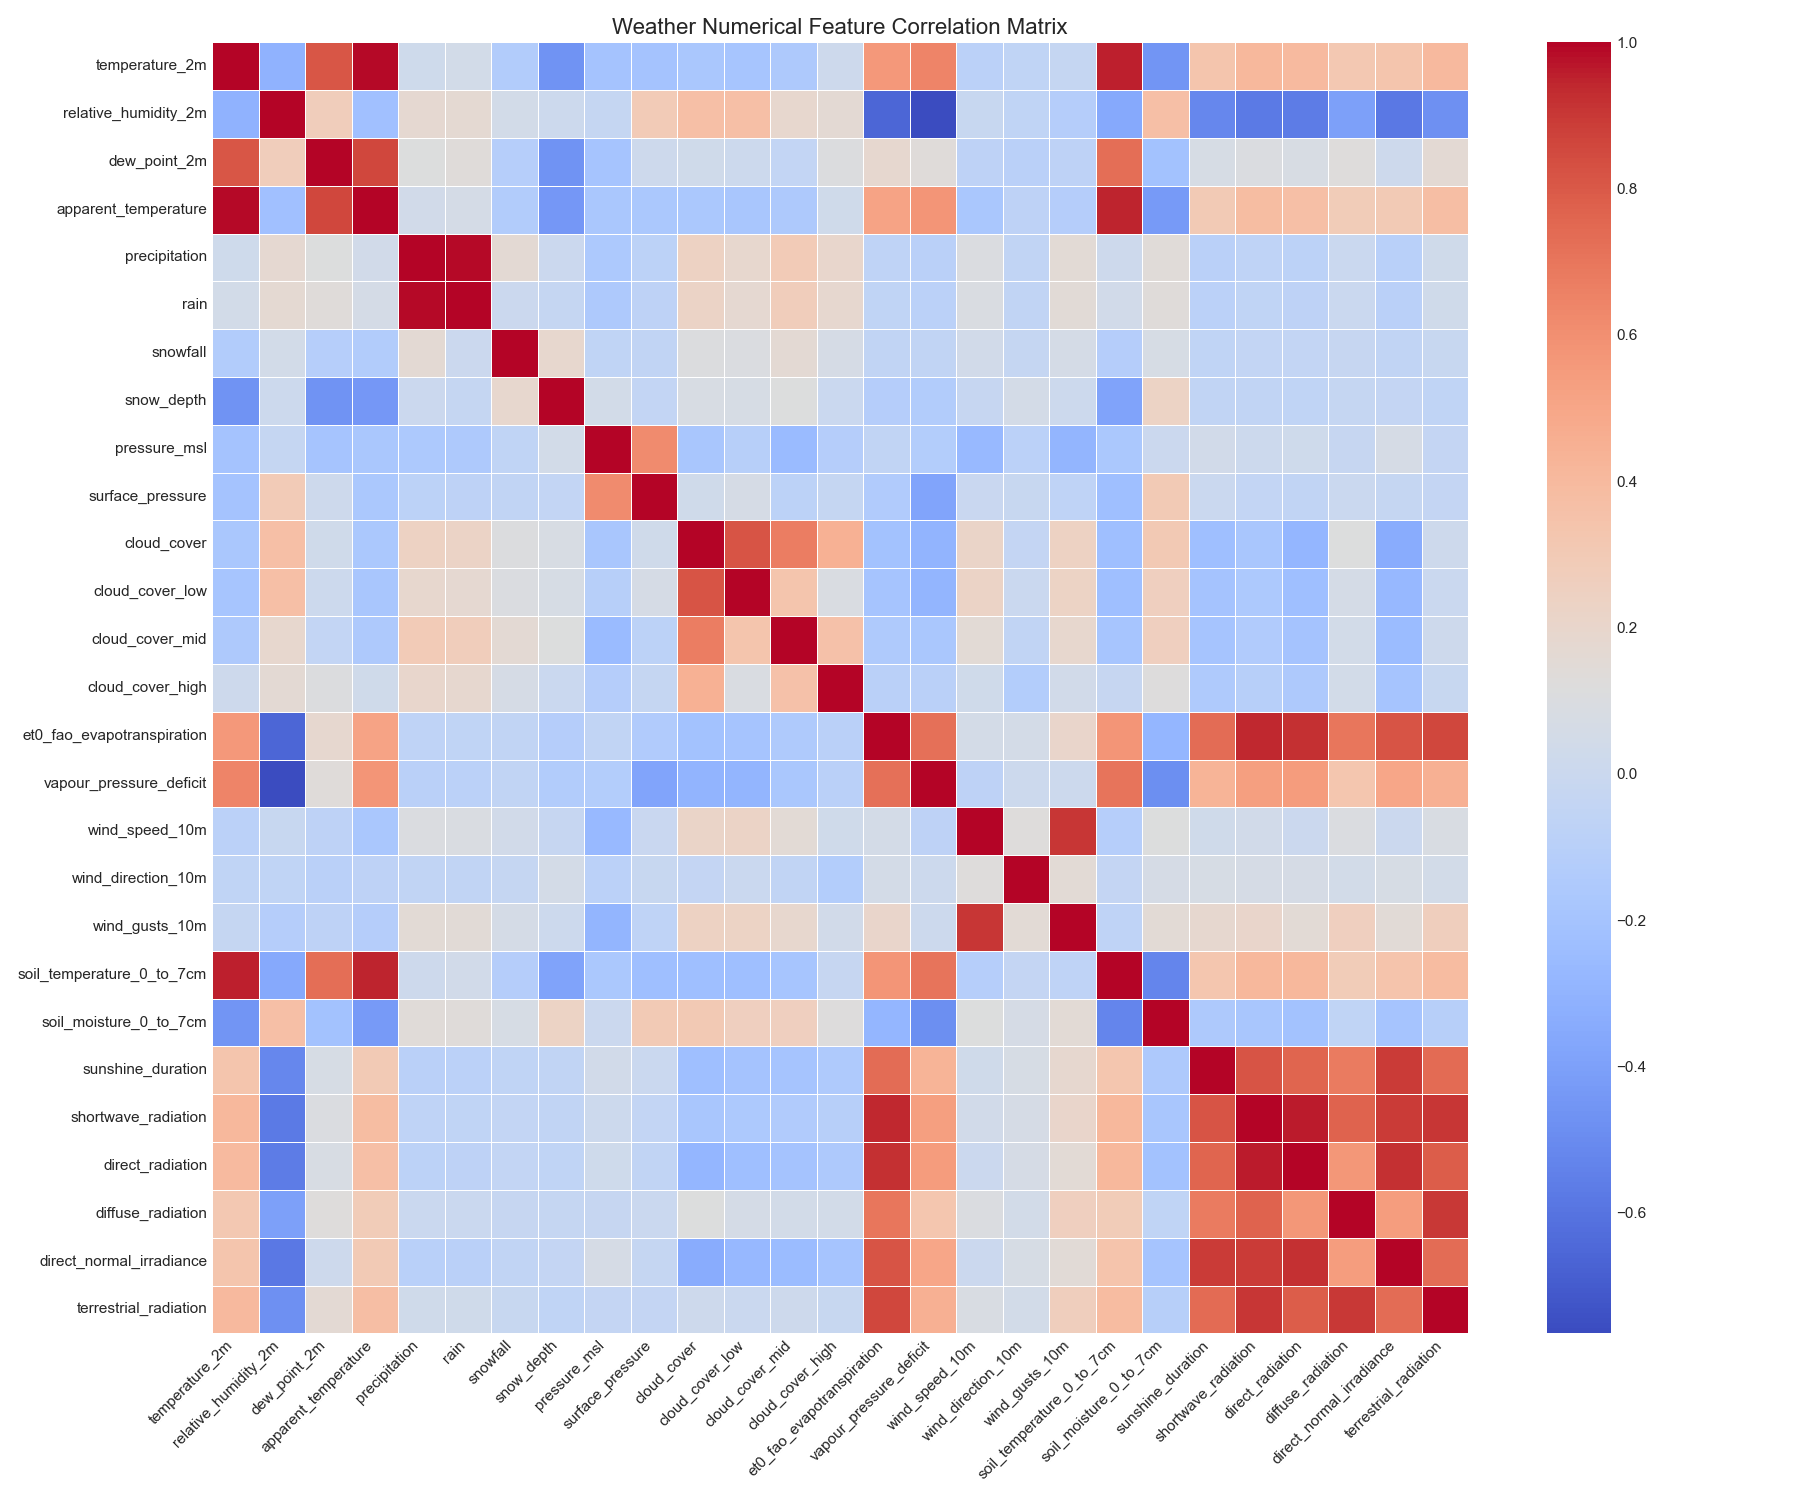
\includegraphics[width=0.8\textwidth]{../plots/weather_correlation_matrix.png}
        \caption{天气特征相关性矩阵}
    \end{figure}
\end{frame}


% 时间特征分析 (与时间频率匹配合并)
\section{时间特征分析与频率匹配} % 合并标题

% 将时间频率匹配和周期性分析的主要发现合并到同一页,图表放在下一页
\begin{frame}{时间特征提取与周期性}
    \frametitle{频率处理与时间模式}
    \textbf{1. 时间频率匹配:}
    \begin{itemize}
        \item Demand 数据频率多样 (15T, 30T, 1H 等),Weather 主要为 1H。
        \item \textbf{处理:} 将需求数据重采样并聚合到小时频率,以便与天气数据合并。
    \end{itemize}

    \textbf{2. 周期性分析:} 需求数据表现出清晰的:
    \begin{itemize}
        \item \textbf{日内周期:} 白天高峰,夜间低谷。
        \item \textbf{周内周期:} 工作日与周末模式差异。
        \item \textbf{年度周期:} 季节性波动 (通常冬夏高)。
    \end{itemize}
\end{frame}

% 将周期性分析的图表放在下一页
\begin{frame}{电力需求平均周期模式}
    \frametitle{平均需求随时间变化}
    % 尝试将三个周期图放在同一页,可能需要缩小或调整布局
    \begin{columns}[T,onlytextwidth]
        \begin{column}{0.48\textwidth}
             \centering
            \begin{figure}
                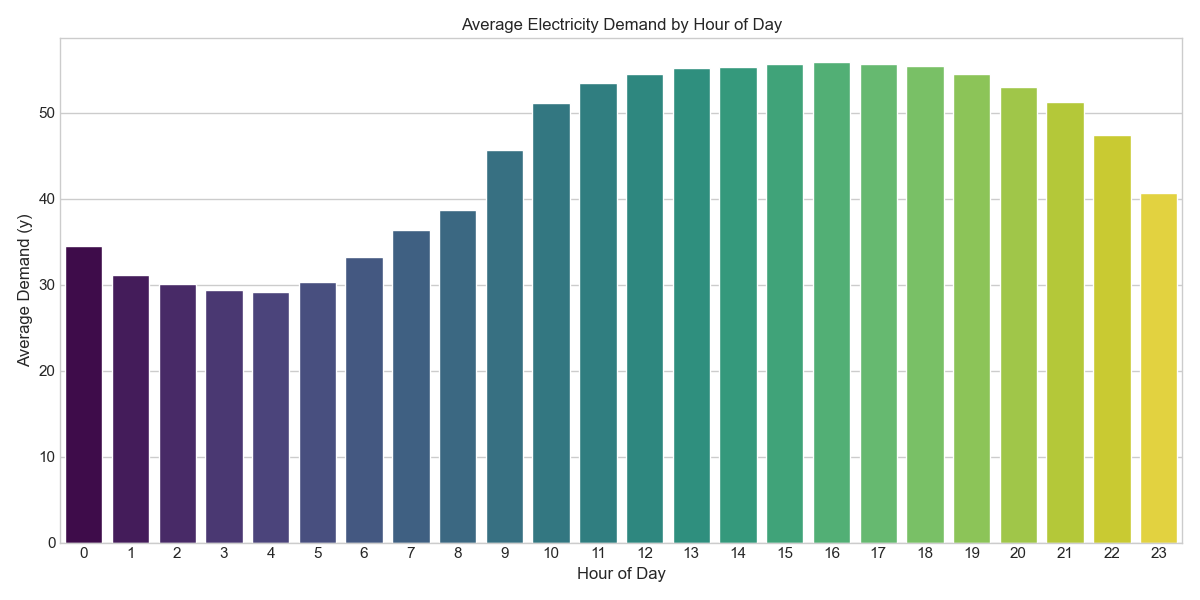
\includegraphics[width=\textwidth]{../plots/avg_demand_by_hour_spark.png}
                \caption{按小时平均}
            \end{figure}
        \end{column}
        \begin{column}{0.48\textwidth}
             \centering
            \begin{figure}
                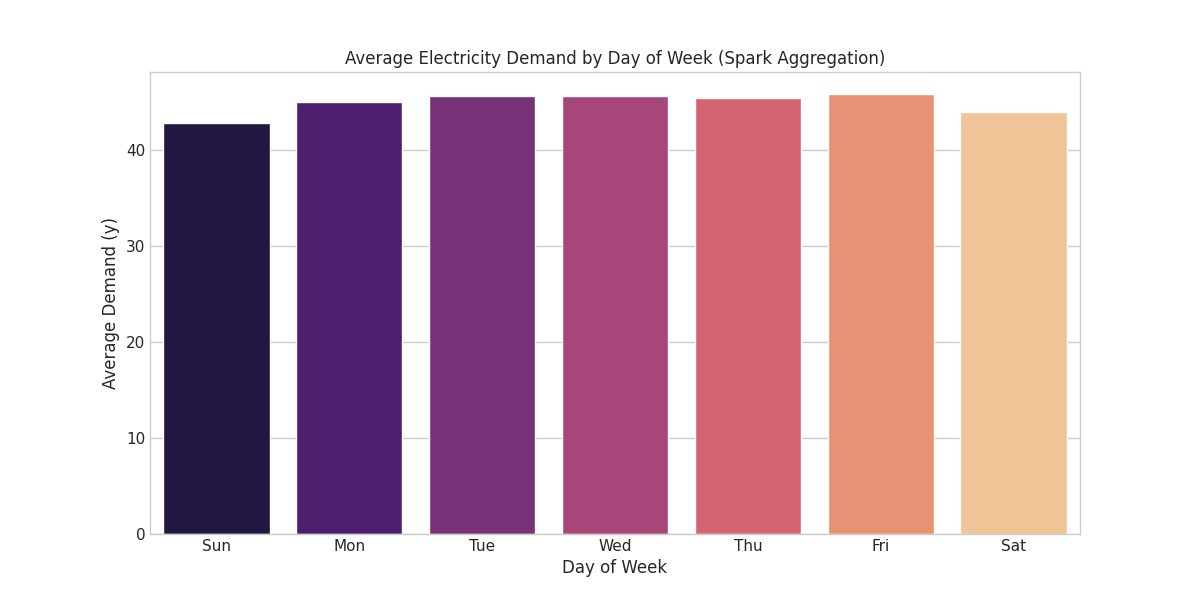
\includegraphics[width=\textwidth]{../plots/avg_demand_by_dayofweek_spark.png}
                \caption{按星期平均}
            \end{figure}
        \end{column}
    \end{columns}
    \begin{figure}[H] % 年月图单独一行或与上面两图调整布局
        \centering
        \begin{figure}
            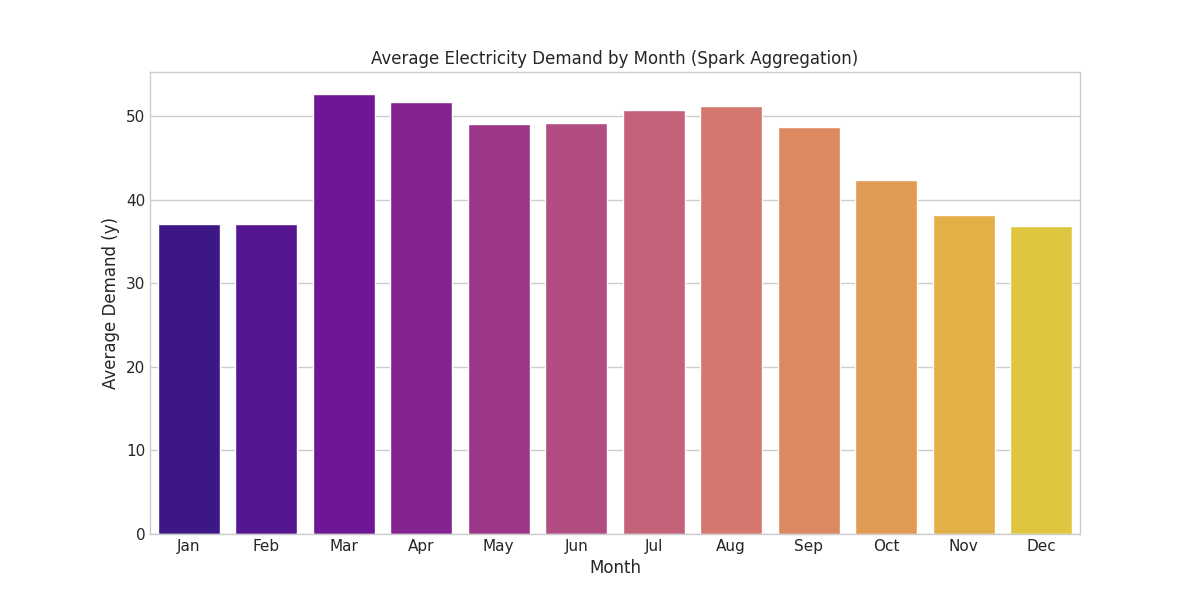
\includegraphics[width=0.6\textwidth]{../plots/avg_demand_by_month_spark.png}
            \caption{按月份平均}
        \end{figure}
    \end{figure}
\end{frame}

% 特征工程
\section{特征工程}
\begin{frame}{特征工程}
    \frametitle{构建预测特征与处理}
    \textbf{1. 特征类型:}
    \begin{itemize}
        \item \textbf{时间特征:} 年,月,日,星期几,年内天,小时。
        \item \textbf{滚动窗口统计特征:} 基于历史需求 (y),窗口 (3H-168H),统计量 (均值,标准差,最小值,最大值)。
        \item \textbf{其他 (来自 Metadata/Weather):} Building Class, Location, Temperature, Humidity 等。
    \end{itemize}

    \textbf{2. 缺失值处理:}
    \begin{itemize}
        \item 移除目标 y 缺失的行。
        \item 移除滚动特征计算初期的缺失值。
    \end{itemize}

    \textbf{3. 特征集输出:} 按年/月分区存储包含原始数据、时间特征、滚动特征的数据集 (`data/features.parquet`)。
    % 将特征工程的两个页面合并为一个
\end{frame}


% 总结与后续步骤
\section{总结与后续步骤}

% 将总结和后续步骤合并,但后续步骤可以分页面展示以保持清晰
\begin{frame}{总结}
    \frametitle{主要发现回顾}
    \begin{itemize}
        \item \textbf{数据特性:} 规模大,异构多源,需求分布高右偏。
        \item \textbf{数据质量:} y 缺失,元数据位置缺失,天气重复 (已处理)。
        \item \textbf{关系:} 建筑类型、天气 (温湿度) 与需求相关。
        \item \textbf{时间模式:} 需求有清晰的日/周/年周期性,时间频率不匹配已通过重采样解决。
    \end{itemize}
\end{frame}

\begin{frame}{后续步骤}
    \frametitle{下一步:模型构建准备}
    \begin{enumerate}
        \item \textbf{数据清洗/预处理:} 处理合并后天气缺失的约 1.73\% 行 (插补或移除)。
        \item \textbf{进一步特征工程 (可选):}
        \begin{itemize}
            \item 滞后特征 (Lag Features)
            \item 交互特征 (Interaction Features)
            \item 分类特征编码 (独热,目标编码等)
            \item 数值特征变换/归一化
        \end{itemize}
    \end{enumerate}
\end{frame}

\begin{frame}{后续步骤}
    \frametitle{下一步:模型选择与评估}
    \begin{enumerate}
        \setcounter{enumi}{2} % 继续编号
        \item \textbf{模型构建准备:} 合理划分训练/验证/测试集 (时序交叉验证)。
        \item \textbf{模型选择与评估:}
        \begin{itemize}
            \item 选择合适模型 (统计,ML, DL)。
            \item 建立完整预测流程 (pipeline)。
            \item 选择评估指标 (RMSE, MAE, MAPE)。
            \item 在验证集上进行模型调优。
            \item 在测试集上进行最终评估。
        \end{itemize}
    \end{enumerate}
\end{frame}


\end{document}
